\begin{figure}[H]
  \centering
  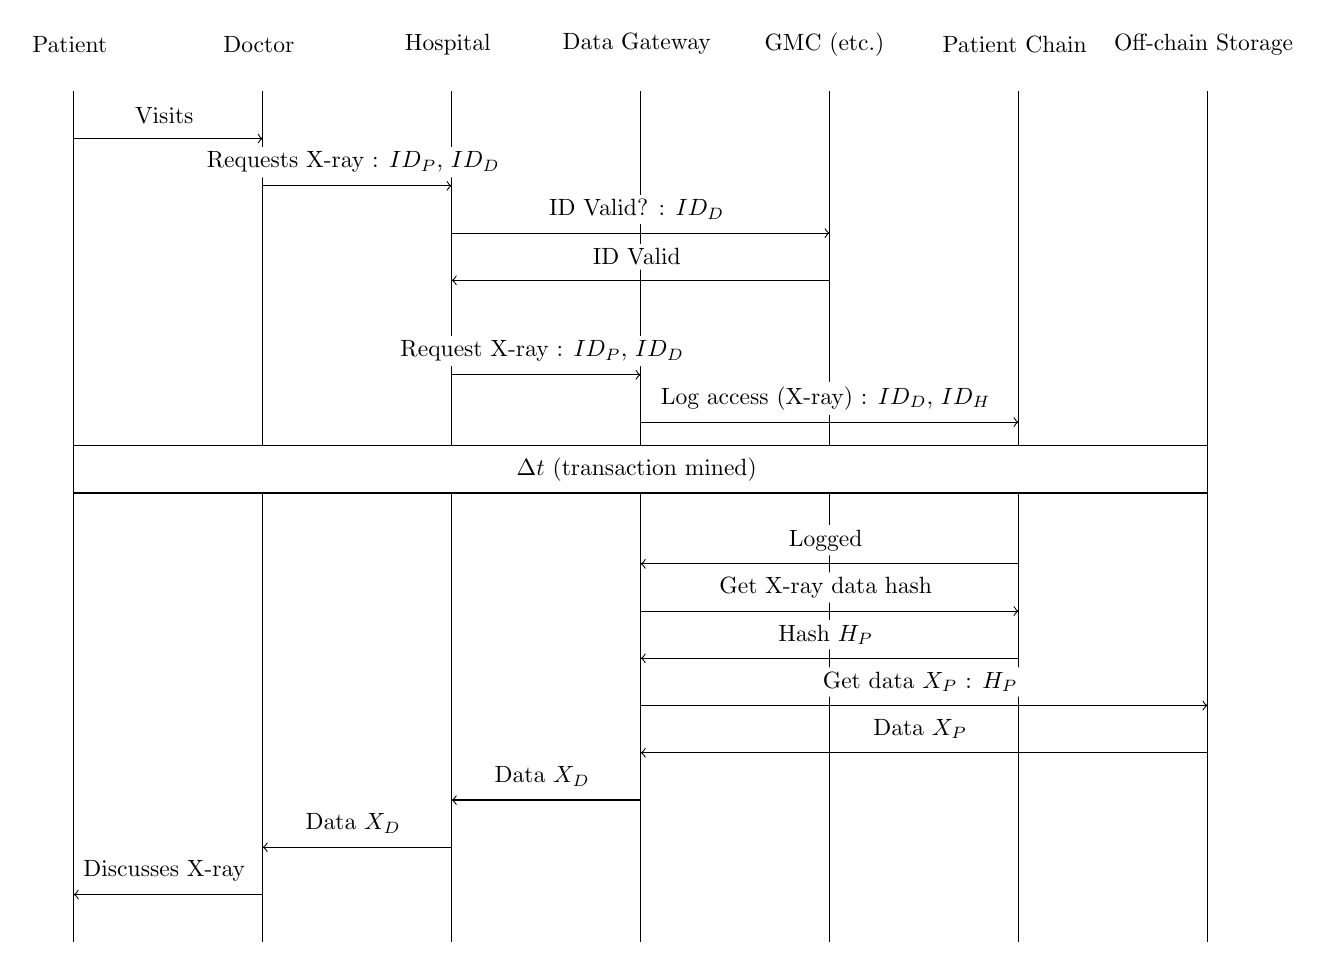
\begin{tikzpicture}[scale = 0.6, every node/.style={scale = 0.85}, every node/.append style={fill = white, rounded corners = 2pt, inner sep = 2pt, align = center}]

  % Lines
  \draw (4, 2) -- (4, 20);
  \draw (8, 2) -- (8, 20);
  \draw (12, 2) -- (12, 20);
  \draw (16, 2) -- (16, 20);
  \draw (20, 2) -- (20, 20);
  \draw (24, 2) -- (24, 20);
  \draw (28, 2) -- (28, 20);

  % Headings
  \node at (4, 21) { Patient };
  \node at (8, 21) { Doctor };
  \node at (12, 21) { Hospital };
  \node at (16, 21) { Data Gateway };
  \node at (20, 21) { GMC (etc.) };
  \node at (24, 21) { Patient Chain };
  \node at (28, 21) { Off-chain Storage };

  % Arrows
  \node at (6, 19.5) { Visits };
  \draw [ -> ] (4, 19) -- (8, 19);

  \node at (10, 18.5) { Requests X-ray : $ID_{P}$, $ID_{D}$ };
  \draw [ -> ] (8, 18) -- (12, 18);

  \node at (16, 17.5) { ID Valid? : $ID_{D}$ };
  \draw [ -> ] (12, 17) -- (20, 17);

  \node at (16, 16.5) { ID Valid \checkmark };
  \draw [ -> ] (20, 16) -- (12, 16);

  \node at (14, 14.5) { Request X-ray : $ID_{P}$, $ID_{D}$ };
  \draw [ -> ] (12, 14) -- (16, 14);

  \node at (20, 13.5) { Log access (X-ray) : $ID_{D}$, $ID_{H}$ };
  \draw [ -> ] (16, 13) -- (24, 13);

  \draw[fill = white] (4, 12.5) rectangle (28, 11.5);
  \node at (16, 12) { $\Delta t$ (transaction mined) };

  \node at (20, 10.5) { Logged \checkmark };
  \draw [ -> ] (24, 10) -- (16, 10);

  \node at (20, 9.5) { Get X-ray data hash };
  \draw [ -> ] (16, 9) -- (24, 9);

  \node at (20, 8.5) { Hash $H_{P}$ };
  \draw [ -> ] (24, 8) -- (16, 8);

  \node at (22, 7.5) { Get data $X_{P}$ : $H_{P}$ };
  \draw [ -> ] (16, 7) -- (28, 7);

  \node at (22, 6.5) { Data $X_{P}$ };
  \draw [ -> ] (28, 6) -- (16, 6);

  \node at (14, 5.5) { Data $X_{D}$ };
  \draw [ -> ] (16, 5) -- (12, 5);

  \node at (10, 4.5) { Data $X_{D}$ };
  \draw [ -> ] (12, 4) -- (8, 4);

  \node at (6, 3.5) { Discusses X-ray };
  \draw [ -> ] (8, 3) -- (4, 3);

  \end{tikzpicture}
  \caption{
    Doctor views X-ray with patient
  }
  \label{fig:user_story_03}
\end{figure}
